\chapter{Produktentwicklung}
\label{sec:produktentwicklung}

\section{Workshop}
Um die zweitrangige Prozedur der Ideenfindung pragmatisch abhandeln zu können wurde ein Workshop mit Brainstorming und anschliessender Diskussionsrunde durchgeführt. Folgende Tabelle zeigt die Favoriten aus einem Pool generierter Ideen.

Die Spalte \emph{Potential} bewertet jede Idee nach subjektiver Einschätzung des Projektteams unter Berücksichtigung folgender Faktoren:
\begin{itemize}
	\item Funktionsumfang
	\item Konzeptionelle und technische Herausforderung
	\item Attraktivität (Für Projektteam)
	\item Attraktivität (Für Studierende des Moduls Internettechnologien)
\end{itemize}

\begin{table}[H]
\tablestyle
\tablealtcolored
\begin{tabularx}{\textwidth}{l X X c}
\tableheadcolor
	\tablehead Idee &
	\tablehead Pro &
	\tablehead Contra &
	\tablehead Potential \tabularnewline
\tablebody
	\textit{\gls{WG}-Aufgabenverwaltung} &
	Viele Studierende identifizieren sich tendenziell damit, da sie selber in einer \gls{WG} wohnen, Faktor \emph{Gamification} sehr interessant &
	&
	\faStar\faStar\faStar\tabularnewline

	\textit{Instant Messenger} &
	Attraktive Features wären realisierbar (Realtime, Websockets etc.) &
	Funktionelle Anforderungen könnten Rahmen sprengen &
	\faStar\faStar \tabularnewline

	\textit{Aufgabenverwaltung} &
	Evtl. gute Verwendung des Produkts &
	``\emph{Gibt's wie Sand am Meer}'', viele bestehende Beispielapplikationen \cite{TodoMVC} &
	\faStar\faStar \tabularnewline

	\textit{Chat} &
	&
	Bereits oft verwendet in bestehender Vorlesung, abgenutzte Thematik &
	\faStar \tabularnewline

	\textit{Forum} &
	&
	``\emph{Gibt's wie Sand am Meer}'' &
	\faStar \tabularnewline
\tableend
\end{tabularx}
\caption{Produktideenpool}
\end{table}

Am verheissungsvollsten wurde die Idee des \gls{WG} Aufgabenverwaltungstool eingeschätzt und gefiel dem gesamten Team von Beginn an ziemlich gut. Die Thematik \gls{Gamification} in einem konkreten Produkt umsetzen zu können eliminierte schlussendlich die letzten Zweifel.

In einem nächsten Schritt wurde die rohe Produktidee mit einem Mindmap weiter ausgebaut und die ersten funktionalen Anforderungen wurden entwickelt. Daneben konnte eine konkrete Kurzbeschreibung sowie das erste Branding für das geplante Produkt formuliert resp. entworfen werden.


\section{Mindmap}
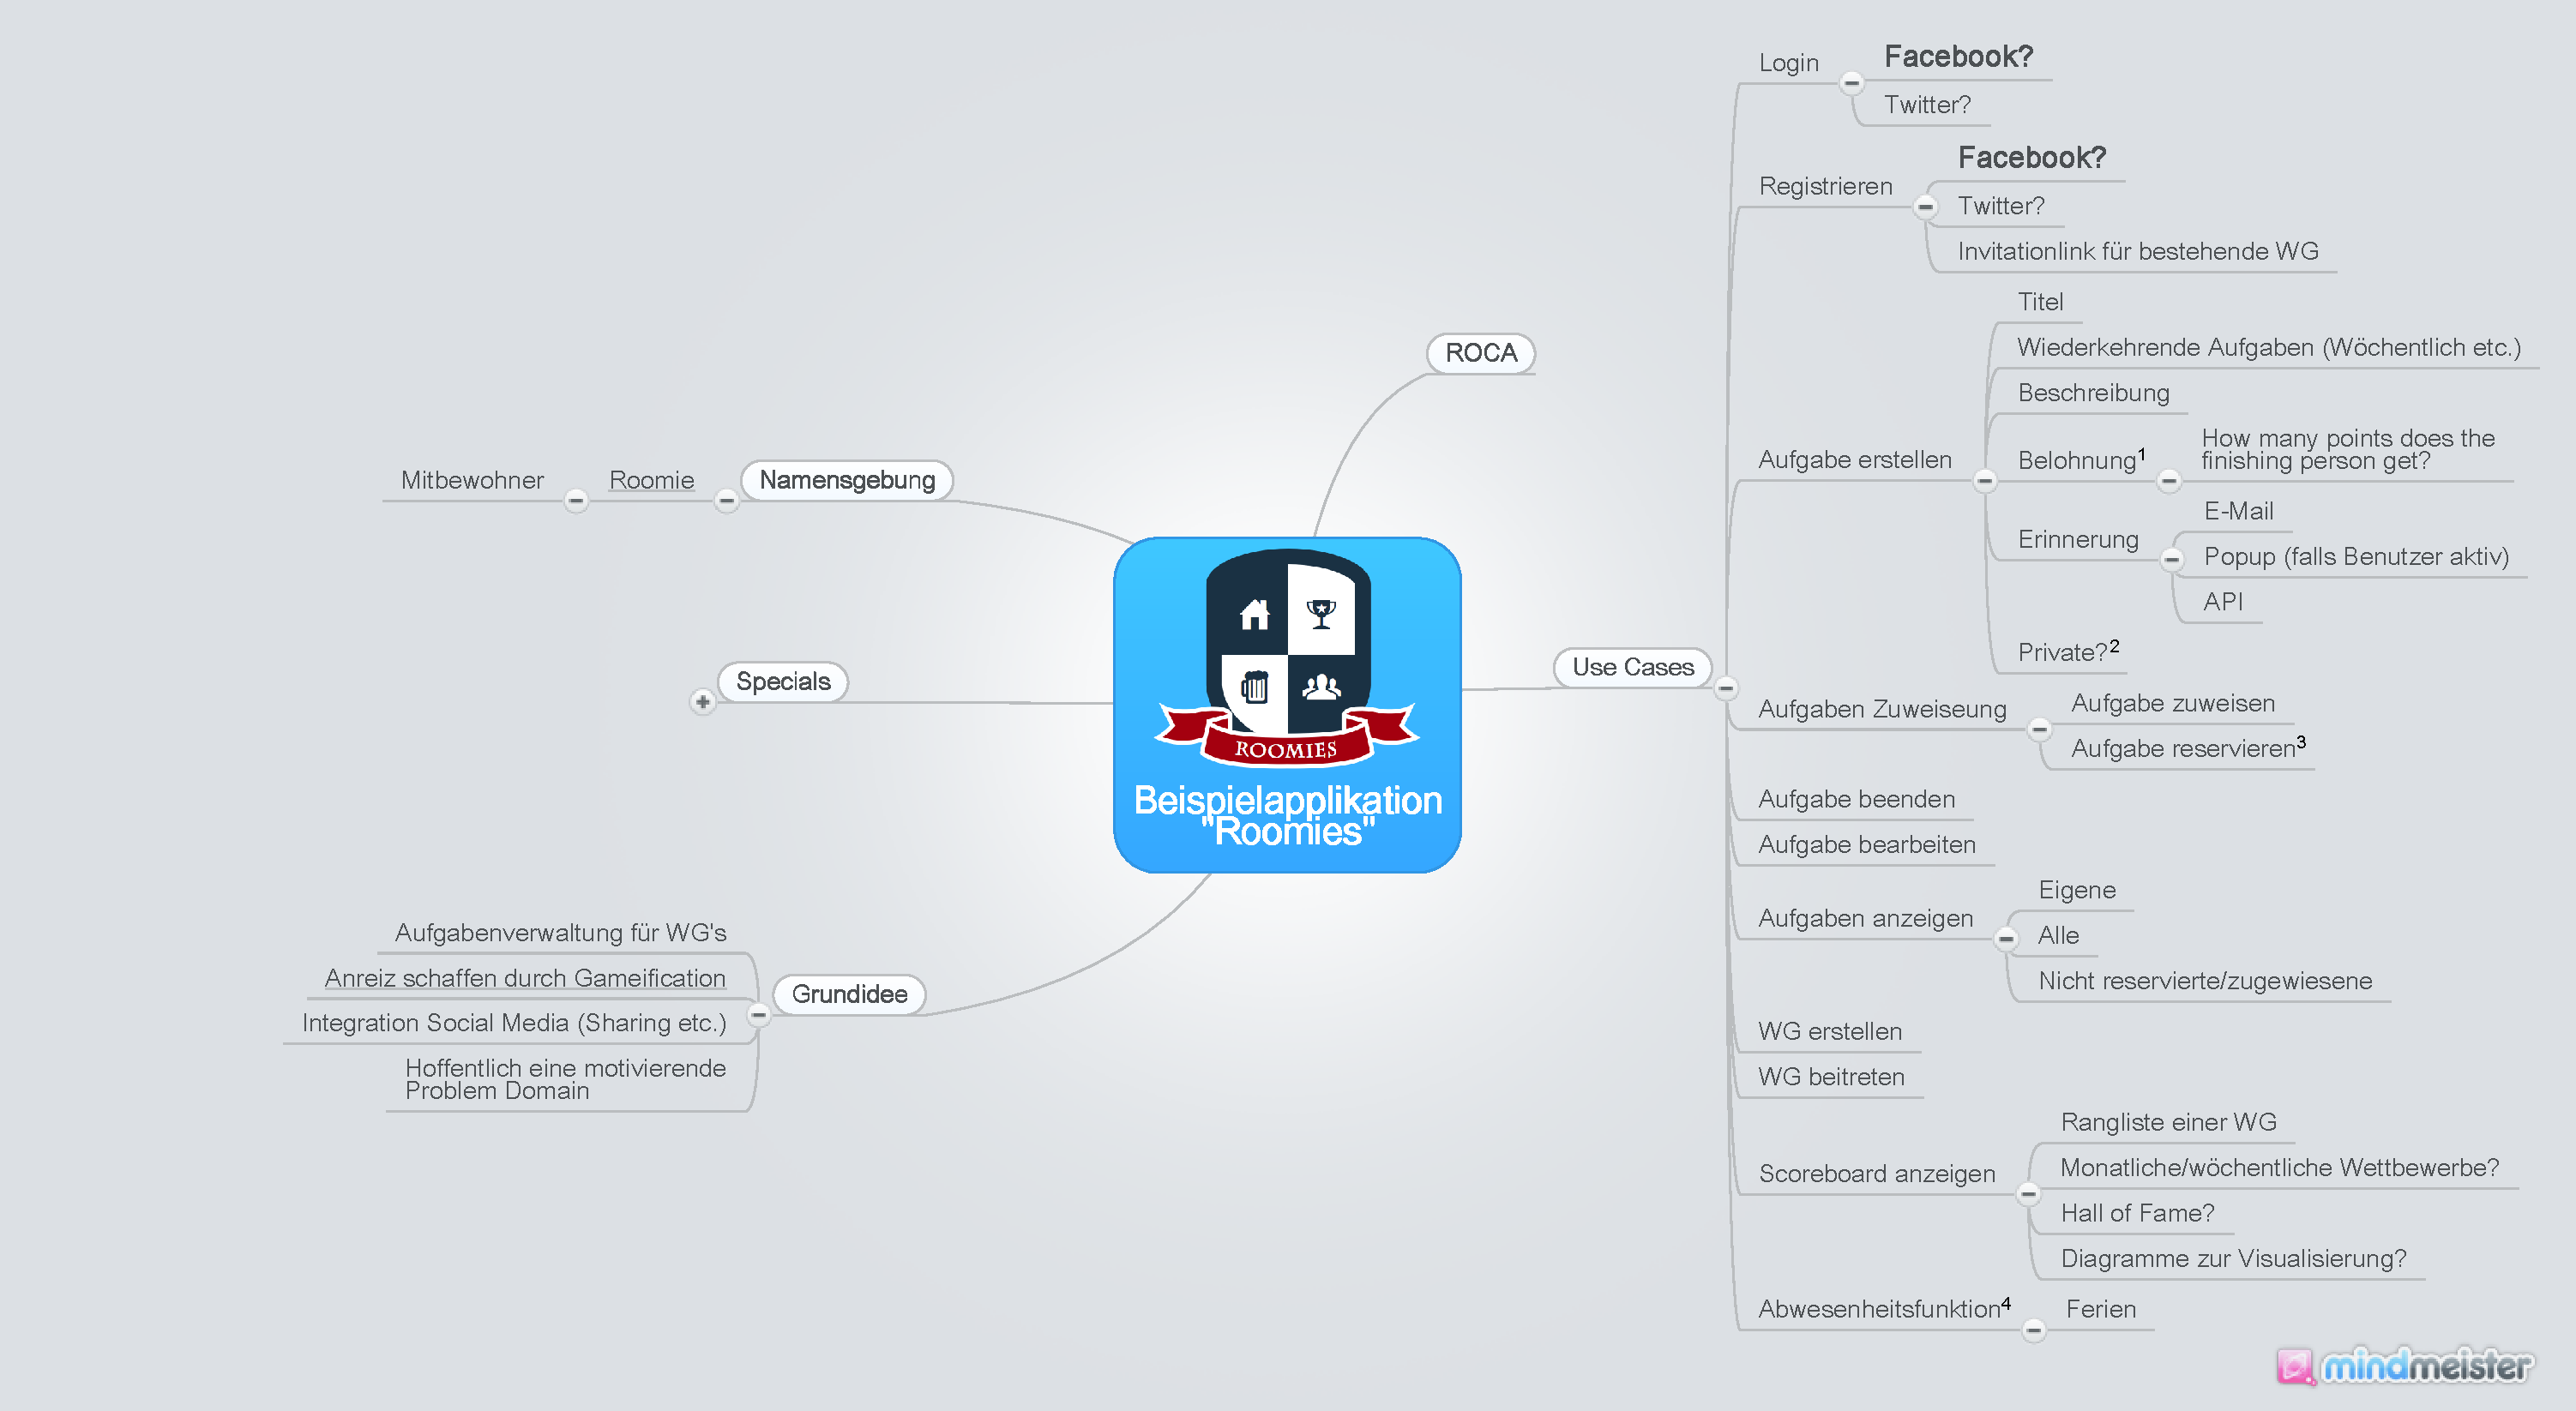
\includepdf[pages=1,pagecommand={},scale=0.75,landscape=true]{content/appendix/mindmap-roomies.pdf}